\documentclass[10pt]{article}
\usepackage{geometry}
\usepackage{setspace}
\usepackage{times}
\usepackage{titlesec}
\usepackage{enumitem}
\usepackage{graphicx}

\titleformat{\section}{\normalfont\bfseries\filcenter}{\thesection. }{0.8em}{}
\titlespacing*{\section}{0pt}{2.0ex}{-1ex}

\titleformat{\subsection}{\normalfont\bfseries}{\thesubsection. }{0em}{}
\titlespacing*{\subsection}{0pt}{2.0ex}{-1ex}

\titleformat{\subsubsection}{\normalfont\it}{\thesubsubsection. }{1.0em}{}
\titlespacing*{\subsubsection}{0pt}{2.0ex}{-1ex}

\geometry{
  a4paper,
  total={165mm,226mm},
  left=20mm,
  right=20mm,
  top=24.5mm,
  textwidth=165mm,
  textheight=235mm
}

\linespread{1.85}

\begin{document}

\noindent \textbf{ABSTRACT:} TODO!

\section{Introduction}
A solid understanding of Data Structures and Algorithms (DSA) is an important skill for any student in the field of Computer Science, since they underpin many of the fundamentals of Computer Science. However, as is the case with many conceptually demanding topics, students can find learning DSA challenging early on in their studies\cite{7600449} due to their inability to correlate DSA concepts with real-world objects and problems. Furthermore, the complexity of DSA means that some students may struggle to engage with the topic, thus requiring more motivation if they are to successfully learn it.\par
Educational tools have often been proposed that either take advantage of Game-based Learning (GBL) or Algorithm Visualisation (AV) in order to help students better learn concepts in computer science.\par
Game-based Learning is the use of games with traditional game elements (such as level progression or animation) in order to teach or practice a particular topic\cite{GBLTeaching}. We find that GBL is been quite commonly used in the some fields of computer science, especially programming, however there are currently few examples of games that directly teach basic DSA. Those games that do exist to teach DSA usually revolve around more advanced DSA theory, such as algorithmic complexity. While learning those concepts are also important, there is a lack of games that help students learn about the practical application of DSA to computer science problems.\par
Another commonly studied educational tool is the concept of Algorithm Visualisation (AV). With AV, we try to abstract away the implementation of a given algorithm or data structure (in terms of, say, memory locations and pointers) and instead present them as static or dynamic diagrams or even analogies. Unfortunately while AVs are commonly seen in DSA teaching, most of these AVs are of the static, box-and-line diagram type\cite{Esponda-Arguero:2010:TVD:1827707.1827710}. When compared to dynamic visualisations that use analogies, static AVs may be less effective at helping students correlate DSA with problems and implementations.\par
We therefore propose an educational tool, DeCode, that integrates both GBL and AV in ways that aren't commonly seen in the field of DSA. By using both GBL and AV approaches, we hope to address both issues with learning DSA - the high complexity (with support from AV), and lack of student motivation (with support from GBL)\par
DeCode is a game-based learning tool for teaching introductory data structures such as Arrays, Lists, Stacks, and Queues alongside basic algorithms that use said data structures. DeCode takes advantage of game-based level design and a 2.5D, animated depiction of data structures. The animation uses the metaphor of cars and parking spaces to better engage the student and help map key DSA concepts to a real-world analogy.\par
The research, implementation process and evaluation of DeCode will be discussed in this report, along with conclusions and possible future work.
\section{Research Intent and Questions}
Our research intent revolves around determining whether our implementation of Algorithm Visualisation with Game-based Learning in the same tool offers improved educational value for students new to learning DSA. We therefore want to address the following research questions;
\begin{enumerate}
  \item Does DeCode help improve students understanding of DSA concepts?
  \item Does DeCode offer additional educational value on top of existing teaching methods or tools (such as box-and-line visualisations of DSA)?
  \item Is DeCode enjoyable and engaging for students to use (and thus students are more likely to remain motivated)?
\end{enumerate}
\section{Literature Review}
\subsection{Algorithm Visualisation Techniques}
One of the first techniques used to improve instruction of DSAs was Algorithm Visualisations. While these were originally limited to drawings on paper and blackboard, these eventually developed into software-generated interactive visualisations as early as 1984, with BALSA\cite{Brown:1984:SAA:964965.808596} as an early example of such. As development progressed, more user friendly visualisation tools were created, with most being freely distributed online as open source software, for use by educators around the world.\par
Despite this work however, the most common examples of AVs are still Static AVs (whether on a computer or paper), which do not allow the user to interact with the visualisation while using it, or allow analogies to be displayed. Recent research has shown that improved interactivity, explanations\cite{vegh2} and the ability for students to construct their own visualisations can help significantly improve the usefulness of AVs to students, especially those that struggle with traditional learning methods\cite{Stasko:1993:AAA:169059.169078}.
\subsection{Existing AV Work}
One of the most prominent algorithm visualisation tools available now is VisuAlgo.net\cite{visualgo}, developed at the National University of Singapore. It offers a clean, modern, 2D visualisation of various data structures, and full interactivity for the user to perform operations on the data structure, and see what happens. The disadvantage of this approach is that the visualisations don't naturally lend to analogies to be constructed. We decided to implement the idea of having interactivity for the user to perform various operations on the data structure into our game, since we felt it allows for much better self-directed learning and experimentation.\par
While most AV tools we identified were designed purely for teaching and demonstration, the TRAKLA2\cite{TRAKLA2} tool was developed to be used as a student assessment tool. Even though it uses similar, traditional representations of DSA as VisuAlgo, TRAKLA adds the ability for students to view algorithm or DS questions. Students are then able to answer the questions by manipulating the visual representation, and have their answer marked automatically. Students are also able to view and browse through (i.e. step back and forward) the model solution for their question.
\subsection{Existing GBL Work}
Despite a large volume of existing work on both Game Based Learning and Algorithm Visualisation, there's a surprisingly low number of papers that implement both GBL and AV to teach DSA. One of the few papers we identified was Park and Ahmed\cite{Park} in which they design a video game using the Unity game engine that visualises various data structures. The game uses real world analogies in order to visualise these in a 3D environment, such as showing the stack data structure as a stack of crates. The player can perform operations on these data structures in order to complete game objectives. Vegh\cite{vegh} presents another similar game that's centred around algorithms rather than data structures. The game uses a real word analogy of crates to demonstrate sorting algorithms (in this case, sort by mass). The game also logs the actions of players, allowing educators to investigate them and determine the student's line of thought.
\subsection{Evaluating GBL}
\label{meegalitrev}
One of the most important steps of building an educational game is the evaluation - we need to know whether our game offers a positive user experience for students, while contributing to learning. It would also help if different educational games can be compared to one another to assess their relative effectiveness. Savi et al presents MEEGA\cite{Rafael}\cite{meegaPlus}, the Model for the Evaluation of Educational GAmes aimed to tackle this. MEEGA is designed to offer a common evaluation model for educational games that can be compared to each other. Its questionnaire model is derived from literature and is designed to measure three dimensions - motivation, user experience and learning. These encapsulate the dimensions of attention, relevance, confidence, satisfaction, immersion, social interaction, challenge, fun, competence and short/long term learning.
\subsection{Other Education Research}
Most tools that teach basic DSA usually don't cover some intricacies of working with them, which can result in students being confused on concepts that might otherwise be regarded as basic. Izu, et al.\cite{izuloop} presents an example of students struggling with array manipulation and loop iterations where students are unable to recognise which direction they should loop in, in order to shift an array to the left or right. They conclude that this is the result of an unintentional oversight in course materials favouring upward loops.\par
Meanwhile, there has also been research into correlations between students ability to explain and trace code and their abilities to write code. Teague and Corney's work\cite{Teague:2012:SHW:2483716.2483727} presents a study of such a relationship where the ability of students to explain a simple code block that swaps two elements is correlated with their ability to explain a simple sorting algorithm that relies on swapping out-of-order elements (similar to BubbleSort).
\section{Goals}
In general, we had three broad goals during the development of DeCode;
\begin{enumerate}
  \item Teach introductory DSA concepts
  \item Be an engaging tool for the user
  \item Offer a highly visually-appealing visualisation
\end{enumerate}
Additionally, from our literature review, we were also able to identify ideas from multiple pieces of existing work that we would like to integrate into DeCode.
\begin{itemize}
  \item An \emph{interactive} algorithm visualisation with explanations, since they've been shown to be more useful to students\cite{vegh2}.
  \item Ask students DSA questions, and allow them to answer them by manipulating the visualisation, such as in TRAKLA2\cite{TRAKLA2}.
  \item Use a game environment, with game objects as real-world analogies to better demonstrate DSes, such as in Park and Ahmed\cite{Park}.
  \item Log students interactions with the tool, to allow educators to better understand student's line of thought, similar to Vegh\cite{vegh}.
  \item Explicitly introduce loop directions and array shifting, since Izu, et al\cite{izuloop} showed that students are commonly confused by this.
  \item Measure students abilities to explain and trace code instead of just their performance in performing DS operations, in order to see if we can reproduce the relationships between the two that Teague and Corney demonstrated in their work\cite{Teague:2012:SHW:2483716.2483727}. 
  \item Evaluate using MEEGA\cite{meegaPlus}, so that we're using a common evaluation model for our game, in order to make it easier to compare our results with other results.
\end{itemize}
\section{Analogy/Metaphor}
\begin{figure}
  \centering
  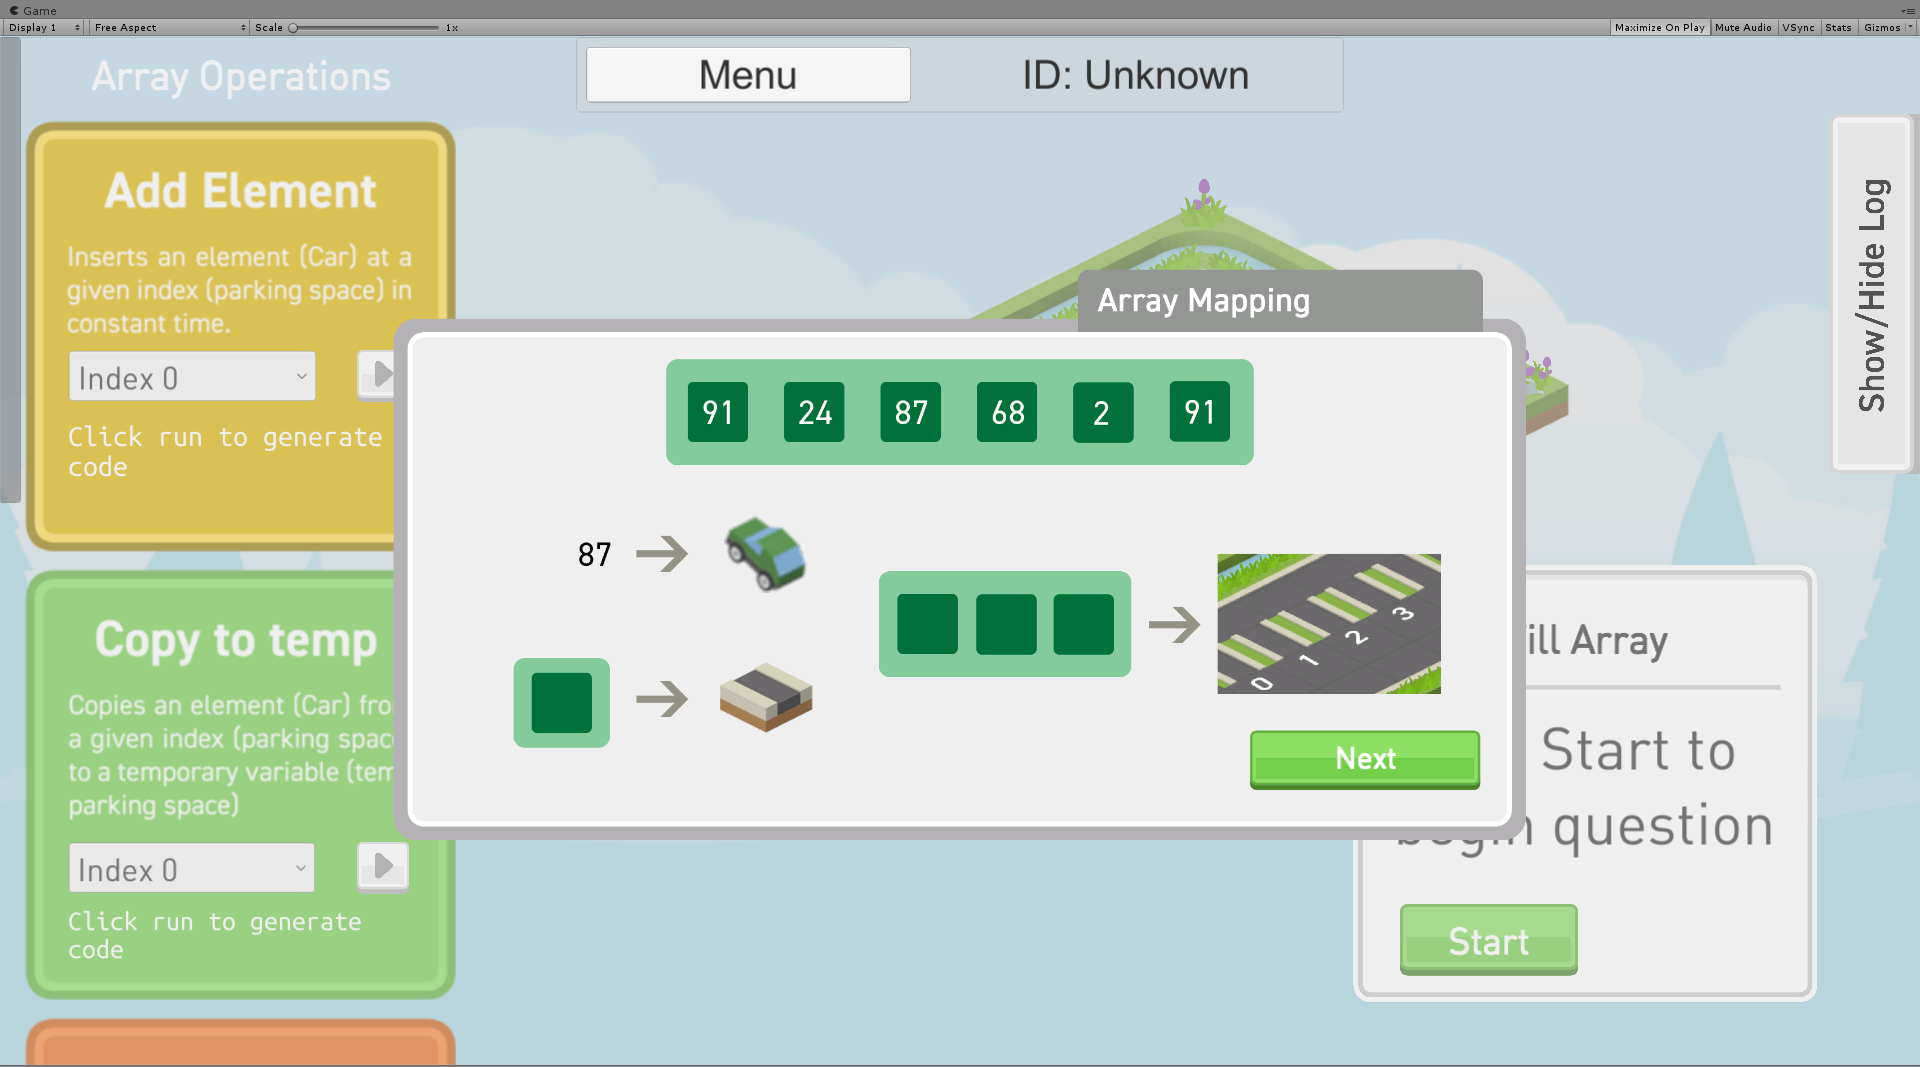
\includegraphics[width=0.75\textwidth]{images/helpanalogy.png}
\caption{Help screen explaining our analogy}
\label{fig:helpanalogy}
\end{figure}
Using an analogy in our visualisation can allow us to make DeCode more visually appealing, while also improving educational value\cite{Park}\cite{vegh2}. However, coming up with an analogy that works for all of our use cases proved to be quite difficult - if something cannot be adequately explained using your analogy, then it quickly falls apart. The analogy should also be relatable for almost all users of the application and not be overly complex. Eventually, we settled on the idea of cars and carparks as our analogy.\par
Cars would represent the values that we would want to store in our data structure, with different types/colours of cars representing different data values that we would like to store. Parking spaces represent locations in memory where these values can be stored, and contiguous blocks of memory (such as arrays) are represented as carparks. To store a value into a memory location, we use the analogy of parking a car into a parking space. The parking spaces are labelled with their index where appropriate.\par
To help users get better accustomed to our analogy, we show a help screen (Figure \ref{fig:helpanalogy})at the start that links the analogy to a more classic box-and-line diagram visualisation of data structures.
\subsection{Limitations}
\label{analogyLimits}
One of our primary goals with this analogy was to have minimal complexity, which meant keeping it to only two main elements (cars and parks). Unfortunately, this meant that there were a few things that ended up being inadequately explained by our analogy.\par
Firstly, the user is able to view the contents of the whole carpark at a time, whereas in reality it takes time to check the contents of each memory location. This made some algorithms such as sorting algorithms more awkward to explain since in reality comparing various indexes makes up a significant portion of the running time of such algorithms. Initially we intended to add some sort of character to the game (such as a driver) to represent the current state of execution - so, as an example, the driver would walk around the carpark and look at cars in order determine their value, then get in one and drive it when array elements are being moved/copied. However, we found that this overly complicated the visualisation, and actually made it harder for users to keep track of what's going on. We therefore decided to go without this, even if it did mean our analogy was less accurate.\par
The second issue was trying to display pointers with our analogy - we simply couldn't come up with something that would fit well that represented a pointer without being overly complex. Signs and other things pointing to a specific parking spot (memory location) would be too complex for students to grasp. Ultimately, we decided to omit most data structures that use pointers, such as Linked Lists since we would be unable to represent them satisfactorily. The only DS that had a pointer was our optimized implementation of Queue, for which we used a red flag to mark the parking space pointed to by a pointer. This only worked since we only had one pointer (having multiple, different coloured flags would be confusing for something like a Linked List).\par
The final issue that we identified was how we would deal with copying of values in the data structure. For example, copying the value from index 0 to index 1 in an array would mean \emph{duplicating} the car that stores the value in index 0 and driving it to index 1, while leaving the original in index 0. This breaks the analogy's link to the real world since one cannot simply duplicate a car in reality. In the end we kept this in the game since we were unable to come up with a way to represent this more realistically. Even if this one part isn't realistic, we feel students will still be able to understand the intent of the analogy.
\section{Design and Technology}
\subsection{Design}
\begin{figure}
  \centering
  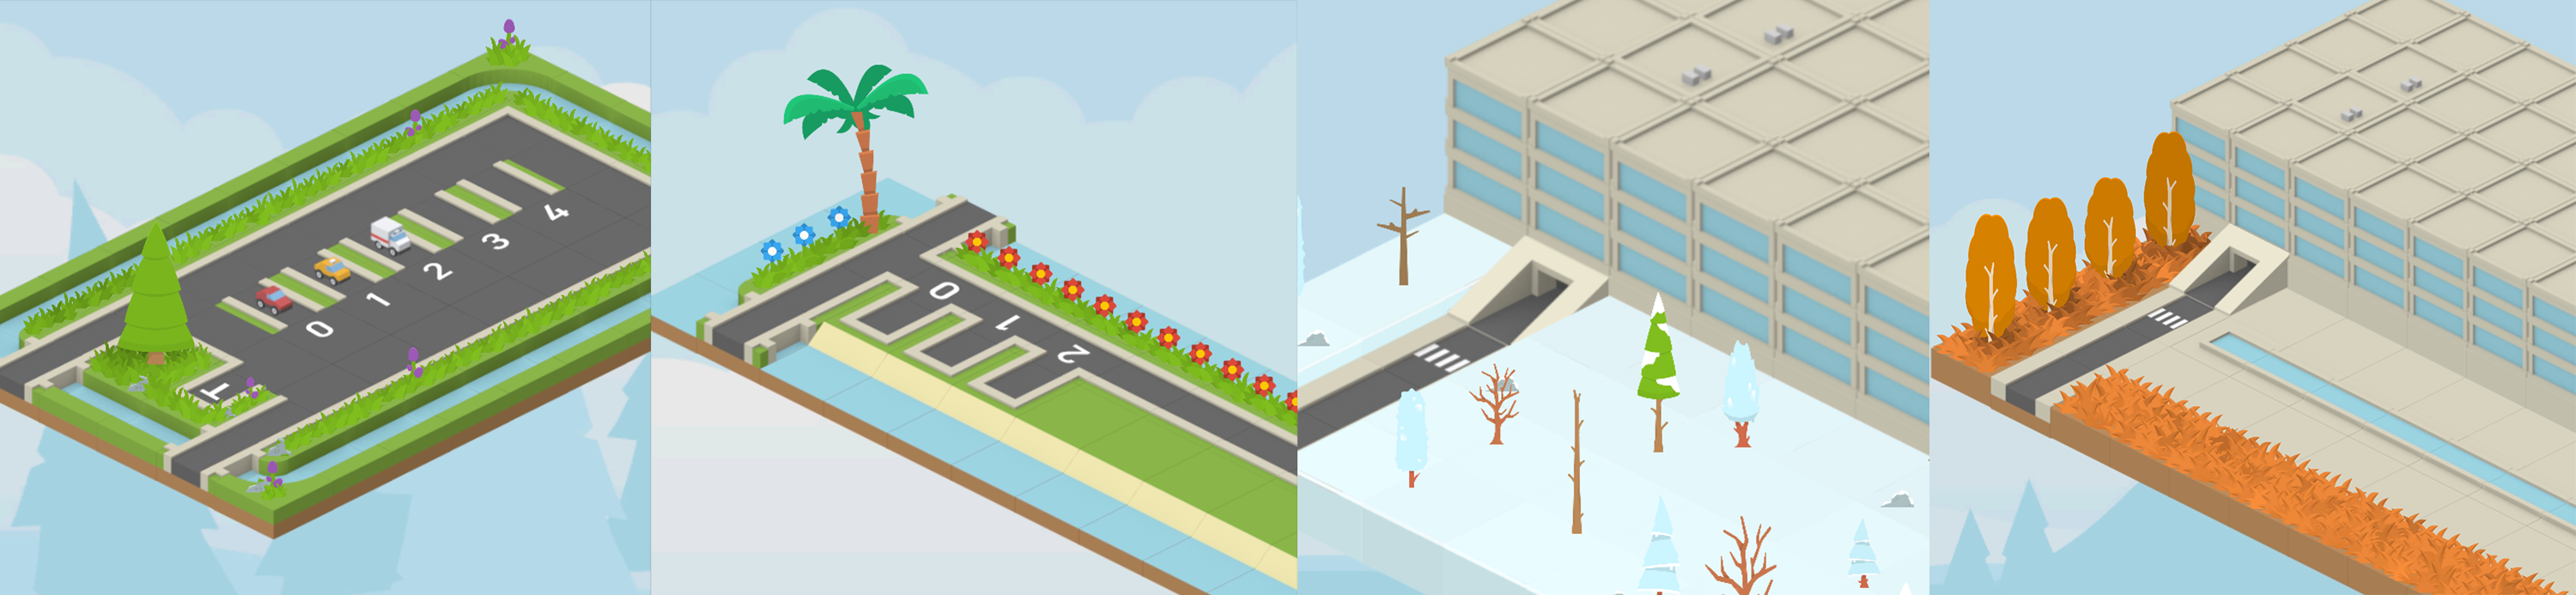
\includegraphics[width=0.5\textwidth]{images/seasons.png}
\caption{4 seasons for the 4 levels in DeCode}
\label{fig:seasons}
\end{figure}
\begin{figure}
  \centering
  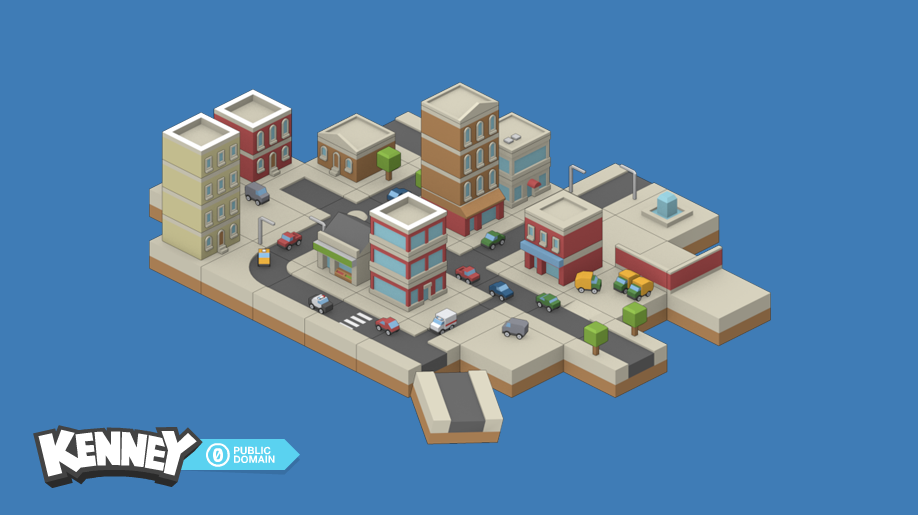
\includegraphics[width=0.45\textwidth]{images/kenneysample.png}
  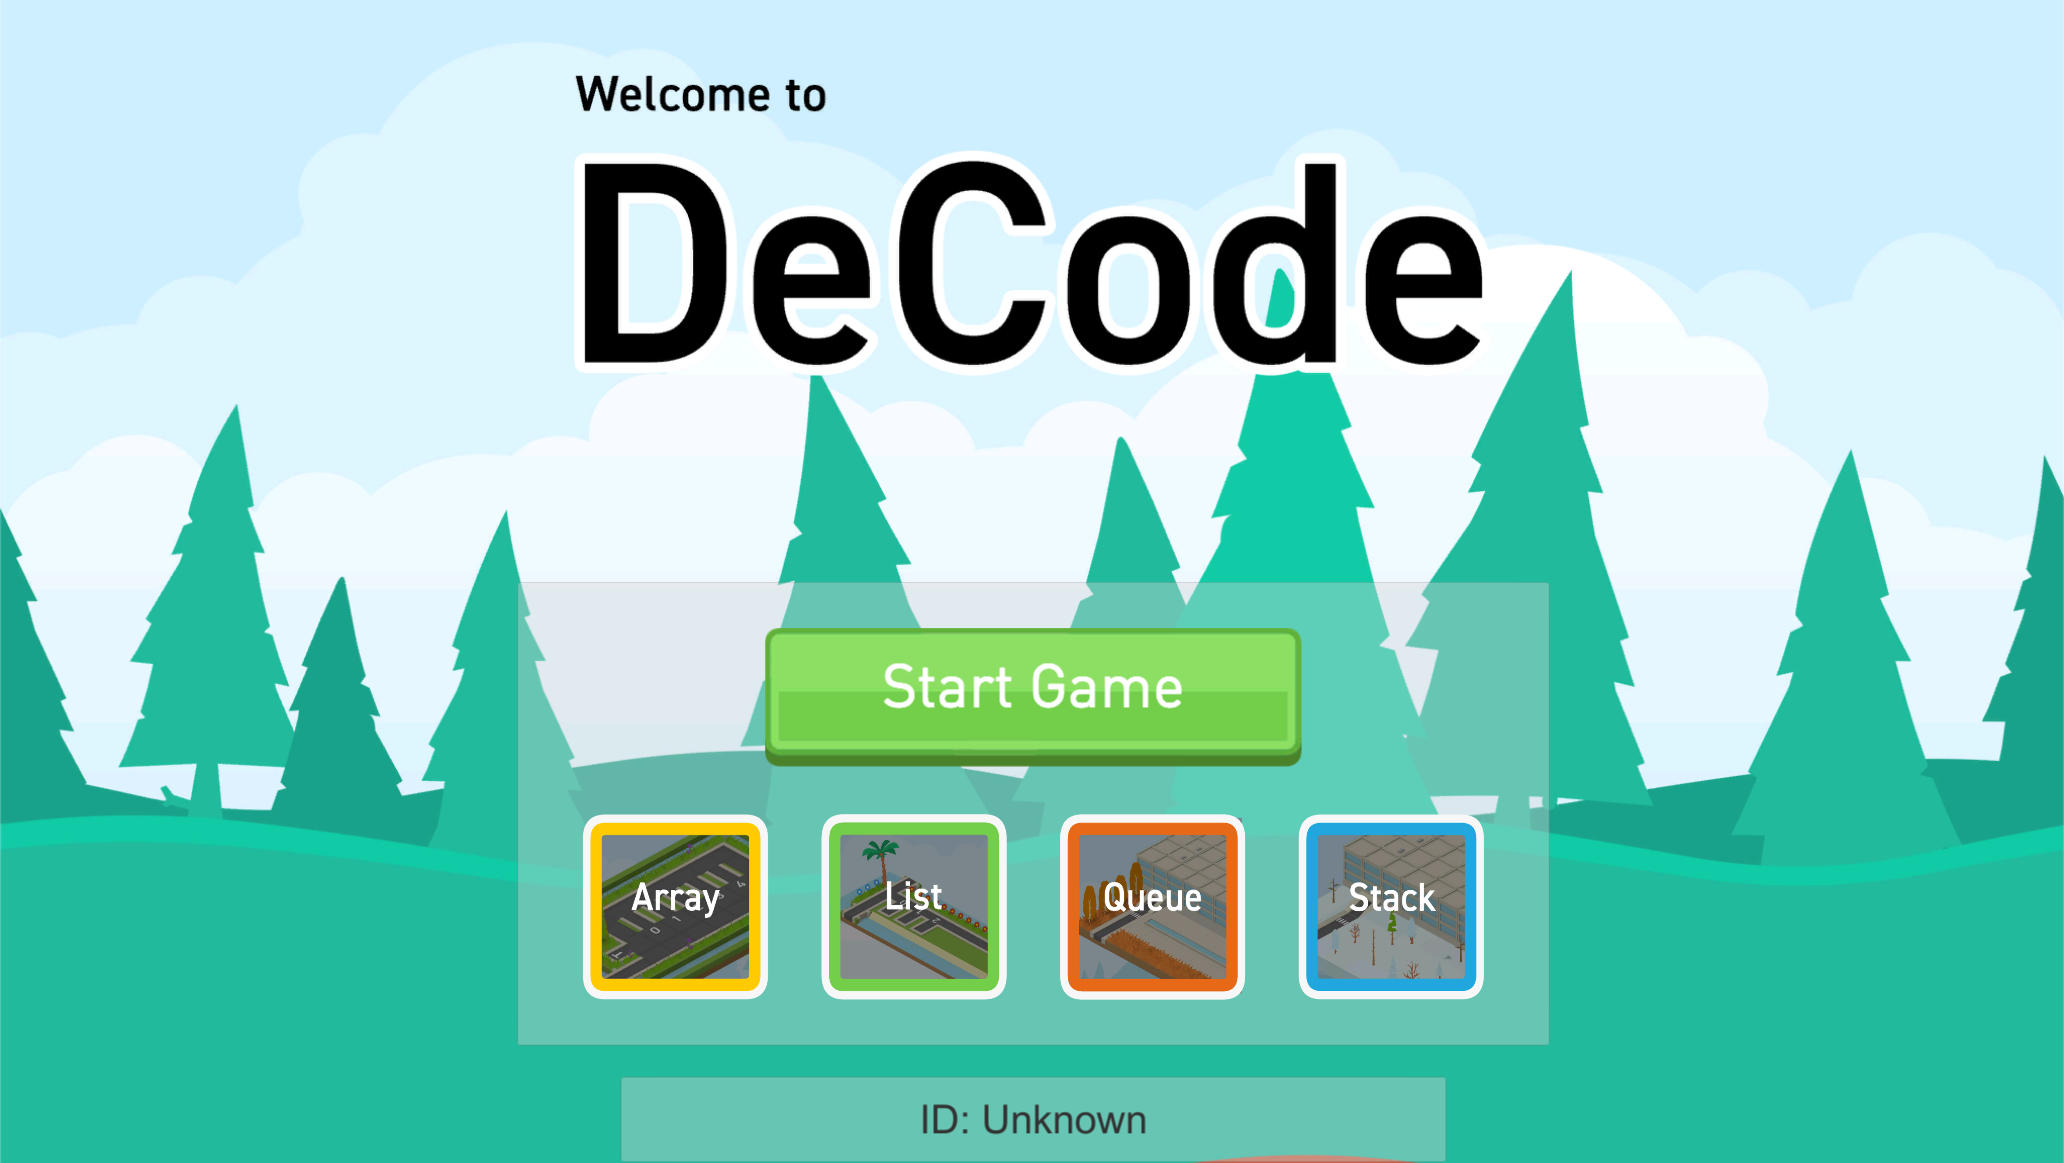
\includegraphics[width=0.45\textwidth]{images/mainmenu.png}
\caption{Left: Sample assets from Kenney's pack, Right: Our main menu UI}
\label{fig:designstuff}
\end{figure}
One of the main goals of DeCode was to design a highly visually appealing visualisations, in order to draw users in and differentiate our visualisation from other, more standard, 2D visualisations. One of the best ways to achieve a high quality visualisation would be to use custom 3D models for our analogies, however we this would've been impractical given the time constraints we were under. Instead, we elected to use existing city assets from Kenney's Isometric City Pack\cite{KenneyAssets}. This asset pack offered most of the assets that we needed for our analogy (city buildings, streets, parking spaces and cars) with a consistent design across them. The assets that weren't available (such as labelled trucks for sorting and indexed parking spaces) were created manually by us, with care taken to ensure they match the design of the Kenney pack.\par
To visually separate each of the 4 data structures we were introducing, each data structure has its own seasonal themed variation on the normal assets. Figure \ref{fig:seasons} shows the design of DeCode across all four seasons (data structures).\par
UI design was also done by us, with the goal of trying to match the design of the Kenney pack as much as possible. A comparison can be see in Figure \ref{fig:designstuff}. Another primary consideration in our UI design was to ensure all UI elements would be usable on a touch device, should a user choose to test our game on such a device. This meant things like array index selection would need to be designed as drop down boxes instead of text boxes, since popping up a keyboard results in a poor touch experience. We also made sure that all buttons were of sufficient size for touch interaction.
\subsection{Technology}
Due to time and cost constraints when developing DeCode, achieving the highest possible technical quality was not a priority in our game. Instead, our choice of technology was largely determined by existing familiarity and cost. With that in mind, we chose to use the Unity game engine\cite{technologies} combined with the Ultimate Isometric Toolkit\cite{isometricToolkit} library - this offered us most of the tools we needed to design our game, with strong existing documentation and 2.5D game support. We were also already familiar with Unity, so we needed less time to get up to speed with the tooling. Unity also supports WebGL deployment, which means DeCode can run in-browser without users having to download anything. Additionally, both of these tools are free (Unity, for non-commercial use) or low cost (Ultimate Isometric Toolkit).\par
% TODO: Do we talk about NodeJS? Not sure if it's relevant.
\section{Data Structures}
We chose 4 data structures to cover in our tool based on their importance in the ACM CS2013 curriculum's section on Fundamental Data Structures\cite{CS2013} and our ability to visualise it using our analogy. As mentioned earlier, we opted to skip data structures that require significant use of pointers since we are unable to represent them using our analogy.
\subsection{Arrays}
Arrays are depicted as a simple carpark of a fixed size, with an extra park representing a temporary variable. Users are asked to fill the empty array and swap values around - this introduces the user to most of the array operations, including add, copying to/from temp and copying from one index to another. Following on, the user is asked to rotate the array using the operations they were just introduced to. We chose to do this since prior work\cite{izuloop} has shown that students are commonly confused by these operations. Finally, we introduce the user to BubbleSort - a common simple sorting algorithm that puts to use all of the operations that they have learned thus far. BubbleSort is introduced in two steps - firstly, users are given an animated demonstration of the algorithm completely with explanations, after which they are asked to step through each step of the algorithm by manipulating the visualisation. Throughout this, the user is asked basic multi-choice questions about what they just did, except in a psuedocode form. This encourages the user to link their knowledge in the visualisation with code.
\subsection{ArrayLists}
\begin{figure}
  \centering
  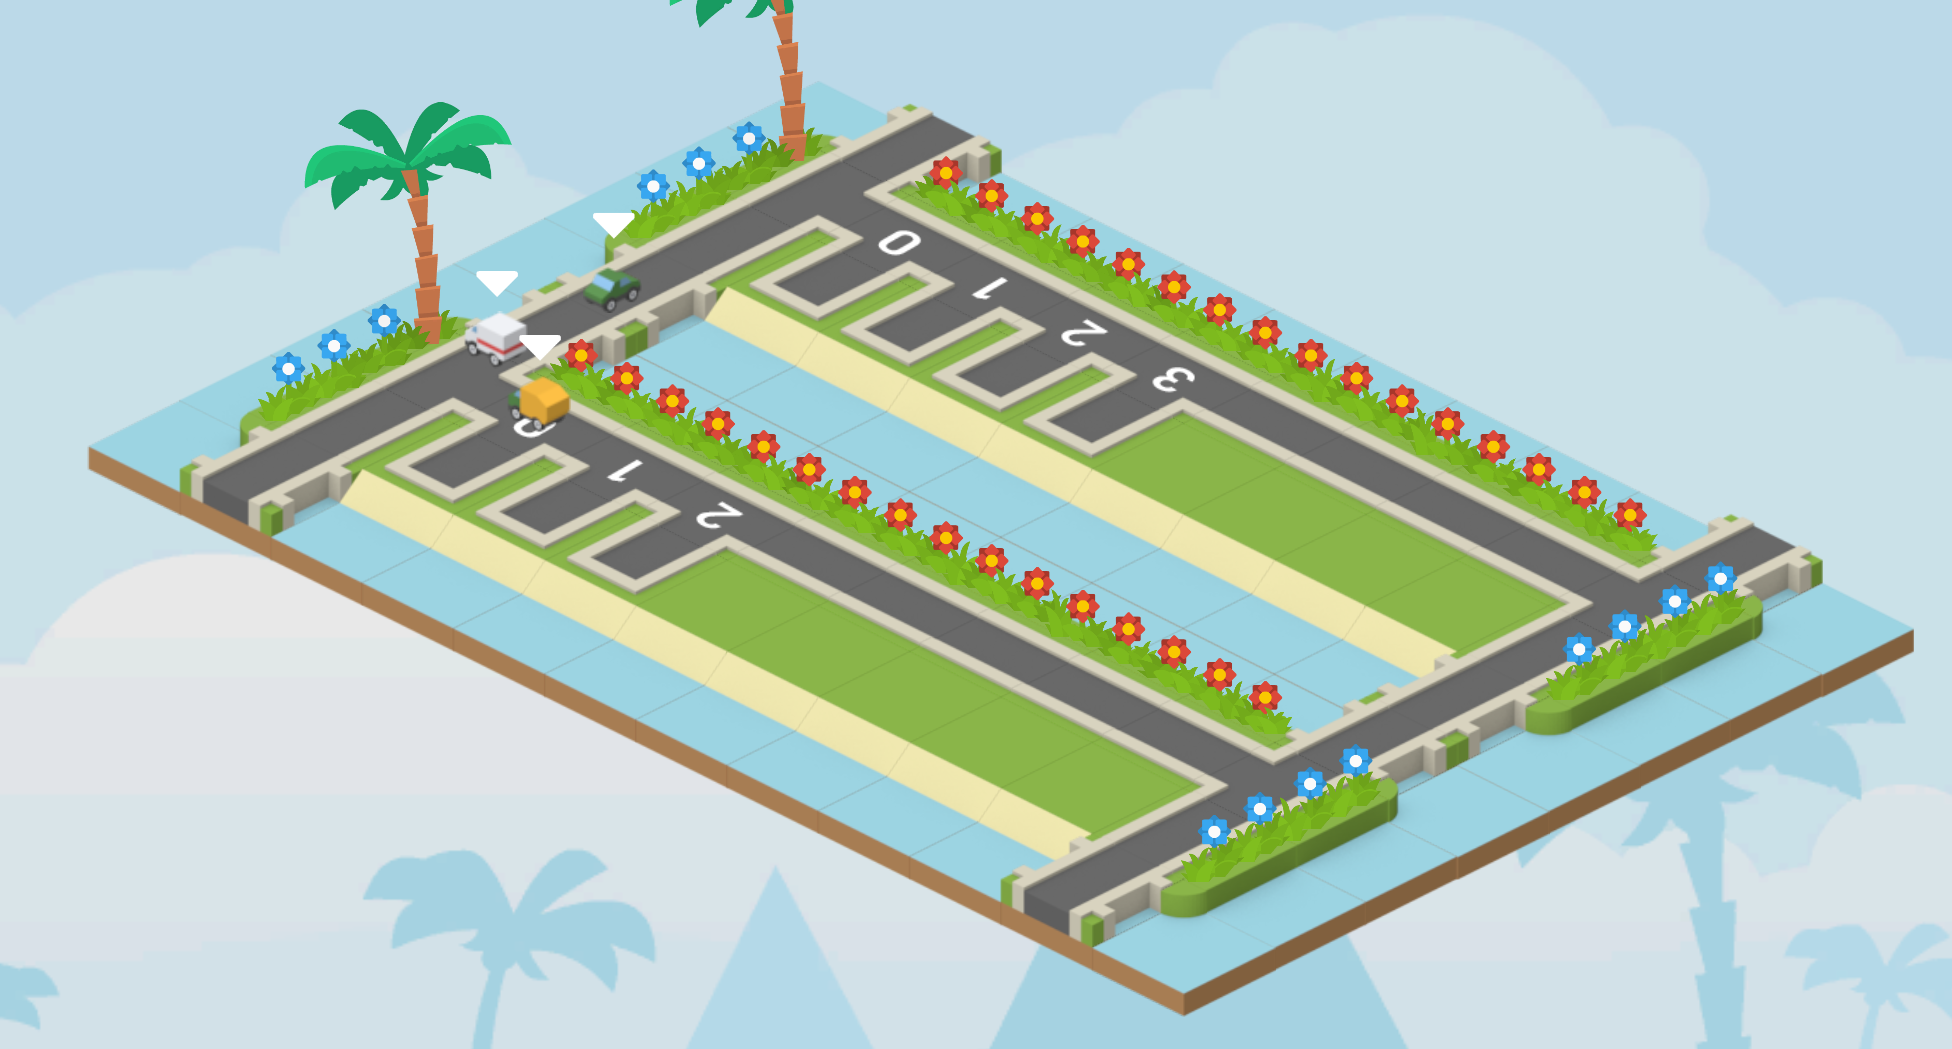
\includegraphics[width=0.7\textwidth]{images/listcopy.png}
\caption{Cars in the middle of being copied to a larger internal array}
\label{fig:listcopy}
\end{figure}
ArrayLists (also known as Vectors in some languages) are introduced in two parts - first, we expose the user to the benefits of a List - namely, dynamic sizing that allows us to add as many elements as we see fit. The user is asked to add elements to the ArrayList, and the internal array is shown as expanding every time a new element is added. This is visualised by having multiple rows of parking spaces next to each other (see Figure \ref{fig:listcopy}), with each row 1 larger than the last. When a new element is added that exceeds the size of the current row, all the cars are moved to the next one, thus representing a possible naïve implementation of ArrayList. Throughout this process, the user is asked questions on how the performance of this implementation could be improved, in order to get them thinking about the next part.\par
In the second part, we introduce a more optimized implementation of ArrayList to the user, in order to give them an idea of how ArrayLists are used in the real world. This done using the same array expanding visualisation as before, except we now show how the implementation doubles the size of the internal array each time.
\subsection{Queues}
% TODO: probably two figures
Since Queues are an abstract data type (ADT), we elected to show it in two parts - first, we show the user the interface of such an ADT, where the implementation is a ``black box'' and the user can only perform enqueue and dequeue operations on said box. We visualise this as a parking garage with one entrance (for enqueues) and one exit (for dequeues). After the user is familiar with these operations, we allow the user to ``see inside'' the parking garage, thus revealing the implementation to them. Similar to ArrayLists, we first introduce them to a naïve implementation of a Queue (basic array), then proceed to introduce a circular array implementation, where we use a pointer (red flag) to arbitrarily define the start of the array.
\subsection{Stacks}
Stacks, being another ADT, are also introduced in a similar way to Queues - first a ``black box'' view where the user can only use the single entrance for push/pop, and then later a ``see inside'' view where the array-based implementation is revealed to the player.
\section{Gameplay Features / User Interface}
\begin{figure}
  \centering
  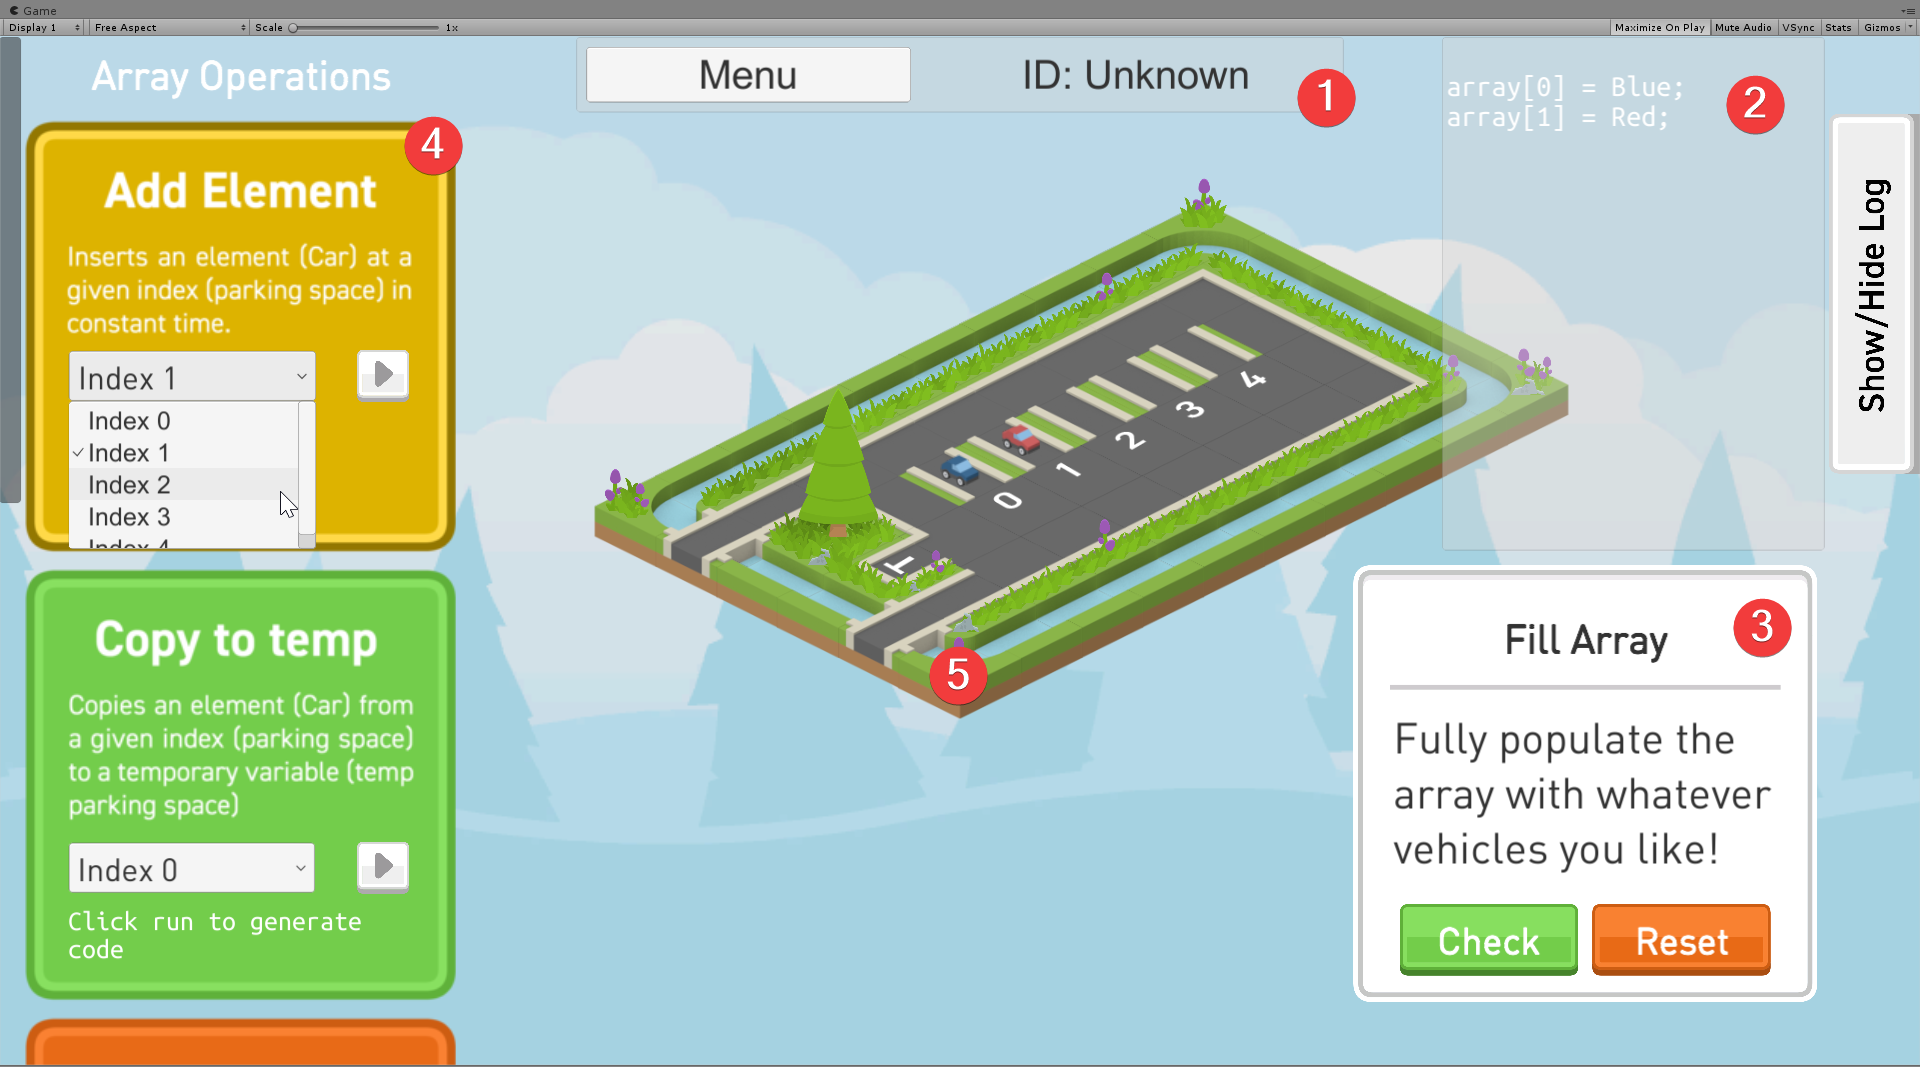
\includegraphics[width=0.75\textwidth]{images/annotatedelements.png}
\caption{Annotated view of the gameplay features}
\label{fig:annotatedelements}
\end{figure}
\begin{figure}
  \centering
  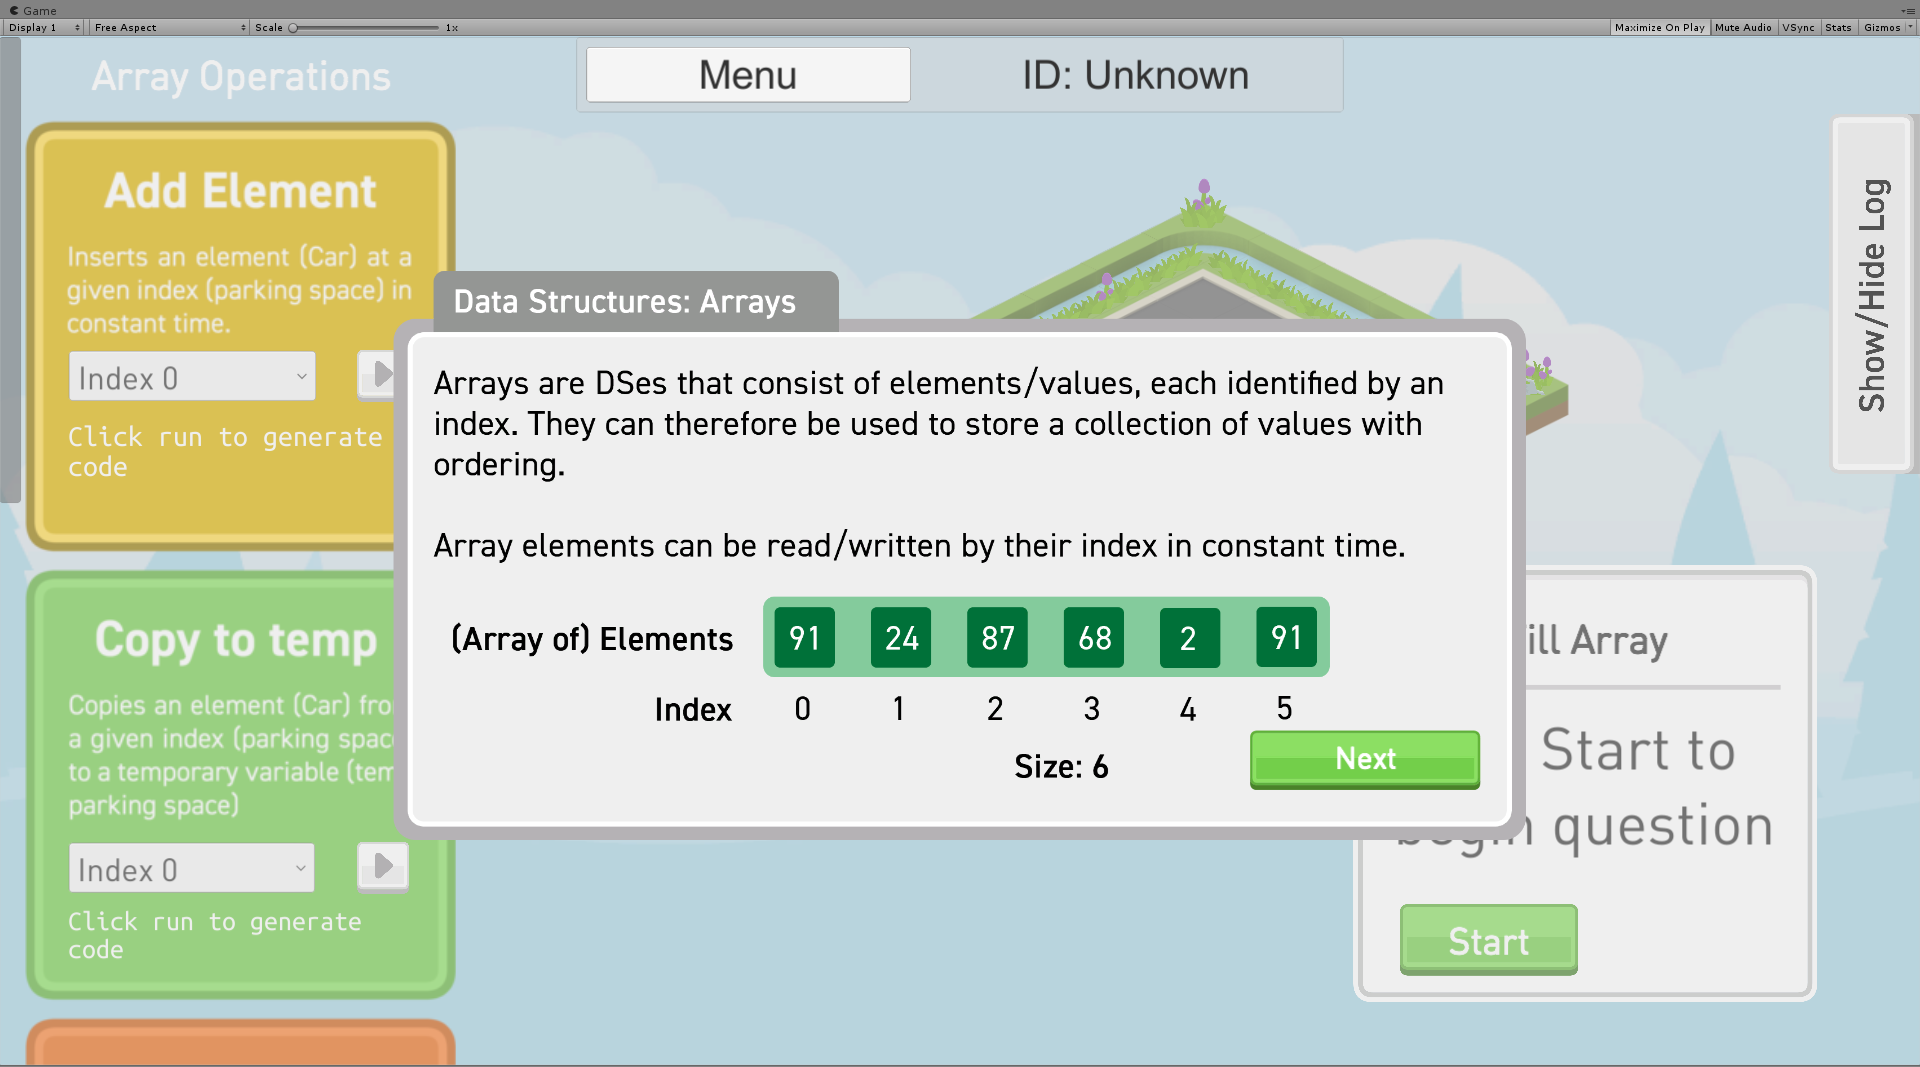
\includegraphics[width=0.48\textwidth]{images/help.png}
  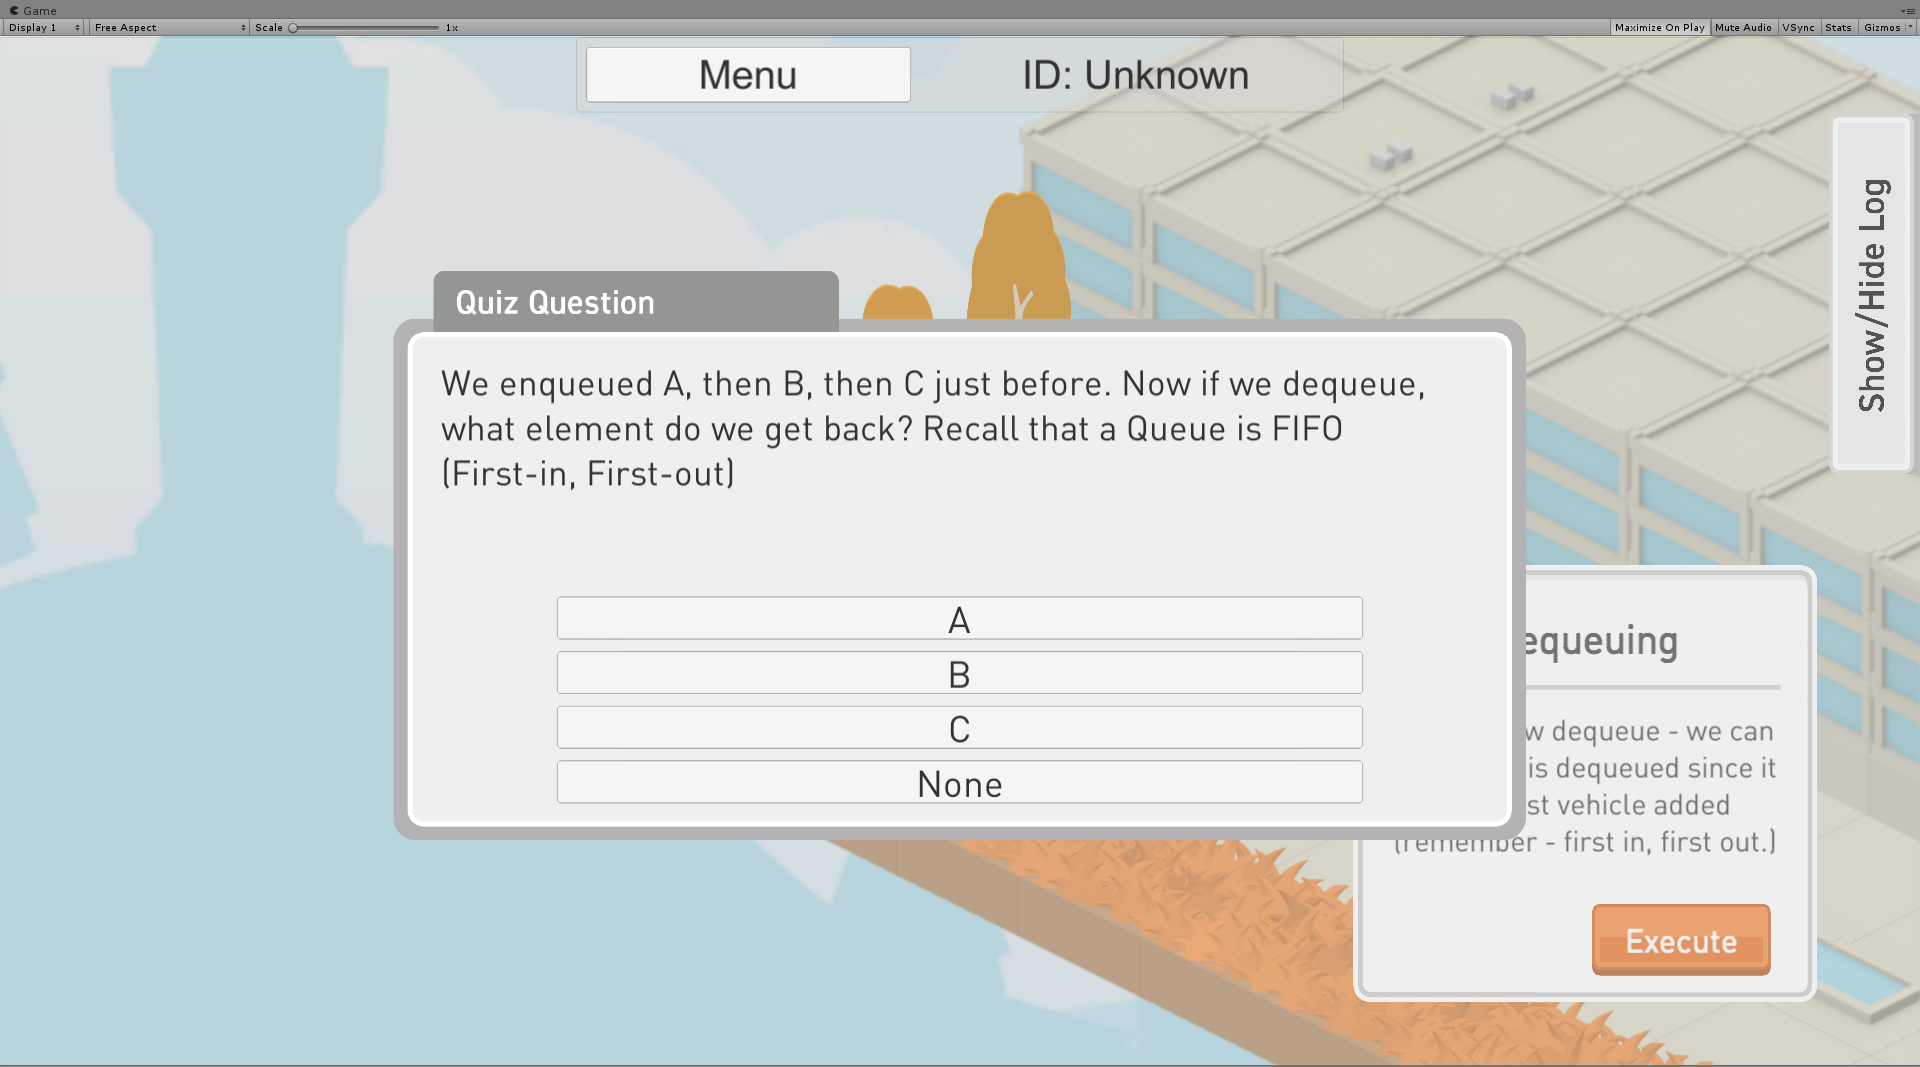
\includegraphics[width=0.48\textwidth]{images/quiz.png}
\caption{The help and quiz pop-up screens}
\label{fig:helpquiz}
\end{figure}
The majority of the game has a interface similar to that shown in Figure \ref{fig:annotatedelements}. The annotated elements do the following\dots
\begin{enumerate}
  \item Shows the user their current game ID, used to track their progress for the evaluation (more in the Evaluation section).
  \item The code view allows the user to see a pseudocode representation of the operations that they have done, so that they can better relate the visualisation with code.
  \item Tasks for the user are introduced here. Users are able to \emph{check} if their answer is correct, or \emph{reset} in order to start again.
  \item Operations supported by the current data structure are shown here, and users can select the index(es) to perform the given operation on. Generally, not all operations are shown at once since they are gradually introduced to the user
  \item The visualisation is shown in the centre of the screen. When the task is introducing something to the user, the visualisation automatically zooms in to focus on what's being shown.
\end{enumerate}
In addition to these elements, DeCode also shows help screens that give users a general introduction to a given data structure, and has quiz screens to ask users specific multi-choice questions, both of which are shown in Figure \ref{fig:helpquiz}.
\section{Evaluation}
\subsection{Design}
In evaluating DeCode, we aimed to answer two main questions, which are related to our research intent - do students enjoy using DeCode, and, if so, is it actually educational?. In order to answer the first question, we rely on a questionnaire answered by students since they have a accurate self-judgement on whether they enjoyed the game or not. For the second question, we rely on a combination of questionnaire answers and in-game data collection, since it's been identified that students have a limited ability to self-assess their learning\cite{Battistella}.
\subsubsection{In-Game}
As students play through our game, data is collected about how long they take to play through each level, what operations they use to perform each task, and how many attempts they take to answer the various multi-choice questions that are displayed. While these statistics are useful in allowing us to know how students are thinking about questions (by looking at their order of operations) or what questions they're struggling on, they don't directly answer our questions about whether DeCode actually offers educational value.\par
In order to help us determine whether students have actually learned anything, we added additional questions into the game where students are asked about similar concepts before and after the game introduces the concept to them. As an example, we asked students to identify the purpose of a piece of swapping code (derived from Teague's work\cite{Teague:2012:SHW:2483716.2483727}) before we introduce the concept to them in the game. We then ask the same question again, except with slightly different naming, afterwards. We intend for this to show possible improvement in knowledge from the student being introduced to the concept in-game. We were unfortunately unable to ask too many of these questions, as we feared it would make the game feel like a test. These questions do, however, introduce a few threats to validity, which we will discuss later.
\subsubsection{Questionnaire}
The primary objective of the questionnaire is to collect data on user's experiences using DeCode, and specifically whether it improves students' motivation by being enjoyable and engaging to use. The original intention was to design our questionnaire around MEEGA\cite{Rafael}\cite{meegaPlus} (more in Section \ref{meegalitrev}), which is designed to measure the user experience and educational value of educational games. However when designing our questionnaire we found that MEEGA (and its sequel, MEEGA2) would take too long for students to answer, and thus result in us getting a reduced response rate to our questionnaire. This is because MEEGA is designed for studies where students must complete the study as part of their course, whereas our study involves students volunteering their own time to participate.\par
In the end, our questionnaire was based around a subset of MEEGA, with most of the questions pertaining to how the students felt about the user experience, and some questions about specific features in the game to gauge their individual usefulness (e.g. the code view or the MCQs).
% TODO: Unfinished!
\subsection{Results and Discussion}
With human ethics and HoD approval, we were able to test DeCode across two different cohorts of students - second-year Mechatronics and Computer Systems engineering students who haven't been formally taught DSA yet, and Software engineering students who had been formally taught DSA in the previous semester. Students were invited to try DeCode and complete the questionnaire in their own time, in exchange for a chance to enter a raffle for a small prize.\par
In the end, approximately 70 attempts were made at DeCode, of which 50 completed at least 
\subsubsection{Questionnaire}

% Direct evidence of students getting better
% Indirect evidence (level times speeding up?)
% Threats to Validity
% Selection bias - are we just targeting students who have a keen interest in edu games? Are these the struggling students we're worried about?
\section{Future Work}
\subsection{Game}
While our evaluation didn't identify any pressing issues that needed to be resolved with DeCode, it did identify a variety of smaller issues such as xxx. Fixing these issues would help refine DeCode into a more polished game, and would significantly improve the user experience.\par
Another major upgrade would be to add new levels/data structures to DeCode to cover all of the Fundamental Data Structures outlined in CS2013\cite{CS2013}. This may be quite difficult as it would require overcoming some limitations in our current analogy (more in Section \ref{analogyLimits})
\subsection{Evaluation}
Due to time and resource constraints, we were regrettably unable to perform an evaluation on the scale that we would've liked. In the future, it would be good to perform an evaluation with a larger sample size (perhaps an entire class studying DSA), and collect better, more concrete, data on whether students learning outcomes are improved by using DeCode. This could be done in a few ways, such as implementing a pre and post-test, or analysing the pass rates of students who did and did not use DeCode, which was done by Mathrani et al\cite{mathrani} in a similar study. A full MEEGA\cite{Rafael} evaluation could also be introduced in order to allow for easier comparisons to be made between DeCode and other educational tools that have been evaluated with MEEGA.
\section{Conclusion}

\begingroup

\section*{References}
  \vspace{2mm}

  % Delete the references header
  \renewcommand{\section}[2]{}

  % Reduce spacing
  \begin{spacing}{1.0}

    \bibliographystyle{IEEEtran}
    \small
    \bibliography{references}

  \end{spacing}

\endgroup
\end{document}